\documentclass[12pt]{article}

\usepackage[utf8]{inputenc}
\usepackage{amsmath}
\usepackage{amssymb}
\usepackage{xcolor}
\usepackage{tikz}

\begin{document}
\paragraph{\Large GBI Definitionen}
\subparagraph{\large Formale Sprachen}
\normalsize
\begin{flushleft}
    Eine formale Sprache $L$ ist eine Menge aus Wörtern. \\
    zB.: $L_{ab} = \{a,b\}$ ist die Sprache mit den Wörtern a und b
    \begin{itemize}
        \item Die Potenz eine Sprache ist definiert als: \\
        \begin{align*}
            L^0 &= \{\epsilon\} \\
            L^{n + 1} &= L \cdot L^n
        \end{align*}
        \item Sprache konkateniert mit eine Sprache ist einfach jede mögliche Kombination der Wörter. Als Beispiel nehmen wir wieder $L_{ab} = \{a,b\}$
        \begin{align*}
            L_{ab} \cdot \{aa,bb\} &= \{aaa,bbb,baa,abb\} \\ \\
            L_{ab}^3 &= L_{ab} \cdot L_{ab} \cdot L_{ab} \\
            &= \{a,b\} \cdot \{a,b\} \cdot \{a,b\} \\
            &= \{aa,bb,ab,ba\} \cdot \{a,b\} \\
            &= \{aaa,aab,bba,bbb,aba,abb,baa,bab\}
        \end{align*}
    \end{itemize}
\end{flushleft}
\subparagraph{\large Mengenlehrer (GBI Niveau :D)}
\normalsize
\begin{flushleft}
    Eine Abbildung $f: X \rightarrow Y$ ist\dots
    \begin{itemize}
        \item \textbf{Injektiv} (Linkseindeutig), wenn jedes Element in der Zielmenge $Y$ höchstens ein Urbild aus der Ursprungsmenge $X$ hat. \\
        \includegraphics[width=0.2\textwidth]{injektiv.png} \pagebreak
        \item \textbf{Surjektiv} (Rechtstotal), wenn jedes Element in der Zielmenge $Y$ mindestens ein Urbild in der Ursprungsmenge $X$ hat. \\
        \includegraphics[width=0.2\textwidth]{surjektiv.png}
        \item \textbf{Bijektiv}, wenn die Abbildung sowohl injektiv als auch surjektiv ist. \\
        \includegraphics[width=0.2\textwidth]{bijektiv.png}
        \item \textbf{Rechtseindeutig}, wenn es für jedes Element in der Ursprungsmenge $X$ maximal ein Zielbild in der Zielmenge $Y$ gibt. \\
        \includegraphics[width=0.2\textwidth]{rechtseindeutig.png}
        \item \textbf{Linkstotal}, wenn es für jedes Element in der Ursprungsmenge $X$ mindestens ein Zielbild in der Zielmenge $Y$ gibt. \\
        \includegraphics[width=0.2\textwidth]{linkstotal.png}
    \end{itemize}
    Relationen die sowohl Linkstotal und Rechtseindeutig sind, nennt man auch Abbildungen. Wenn das gegeben ist kann man eigentlich erst $f: X \rightarrow Y$ schreiben.
    $Y$ ist dann der Zielbereich/die Zielmenge und $X$ ist der Definitionsbereich/die Ursprungsmenge
\end{flushleft}
\subparagraph{\large RegEx}
\normalsize
\begin{flushleft}
    Wissenswertes:
    \begin{itemize}
        \item Hilfssymbole $:=$\textcolor{red}{$\{|,(,),\ast,\emptyset\}$}
        \item "$\ast$ vor $\cdot$ (Konkatenation)"
        \item "$\cdot$ vor Strich "$|$" (Oder)
        \item $\langle R \rangle$ ist die formale Sprache, welche mit $R$ gebildet werden kann
        \item $\langle \emptyset \rangle = \{\}$
        \item $\langle R_1| R_2 \rangle = \langle R_1 \rangle \cup \langle R_2 \rangle$
        \item $\langle R_1 \cdot R_2 \rangle =\langle R_1 \rangle \cdot \langle R_2 \rangle$
        \item $\langle R \ast \rangle = \langle R \rangle ^\ast$
        \item Es gibt \textbf{kein} $R+$ sondern $RR\ast$ Bsp.: Statt $(ab)+ \text{ einfach } ab(ab)\ast$
    \end{itemize}
    Bsp.: \\
    $R = a|b$ dann ist:
    \begin{align*}
        \langle R \rangle = \langle a | b \rangle = \langle a \rangle \cup \langle b \rangle = \{a\} \cup \{b\} = \{a,b\}
    \end{align*}
    $R = (a|b)\ast$ dann ist:
    \begin{align*}
        \langle R \rangle = \langle (a|b)\ast \rangle = \langle a | b \rangle^\ast = \{a,b\}^\ast
    \end{align*}
    $R = (a\ast b\ast)\ast$ dann ist:
    \begin{align*}
        \langle R \rangle &= \langle (a\ast b\ast)\ast \rangle = \langle a\ast b\ast\rangle^\ast \\
        &= (\langle a\ast\rangle\langle b\ast\rangle)^\ast = (\langle a\rangle^\ast\langle b\rangle^\ast)^\ast = (\{a\}^\ast\{b\}^\ast)^\ast \\
        &= \{a,b\}^\ast
    \end{align*}
\end{flushleft}
\subparagraph{\large Graphen}
\normalsize
\begin{flushleft}
    \vspace{0.5cm}
    \begin{itemize}
        \item Ein gerichteter Graph ist das Paar \textcolor{red}{$G = (V,E)$}
        \begin{itemize}
            \item \textcolor{red}{Knotenmenge $V$} ist endlich und nichtleer (V für engl. vertex)
            \item \textcolor{red}{Kantenmenge $E$} $\subseteq V \times V$  (E für engl. edge)
            \begin{itemize}
                \item muss damit auch endlich sein, darf aber leer sein
            \end{itemize}
        \end{itemize}
        \item \textcolor{red}{Pfade} können über mehrer Kanten führen
        \item \textcolor{red}{$V^{(+)}:$} Menge der nichtleeren Listen von Elementen aus V
        \item Ein Pfad ist \textcolor{red}{$p=(v_0,\dots ,v_n) \in V^{(+)}$} wenn für jedes $i \in \mathbb{Z}_n$ gilt: \textcolor{red}{$(v_i,v_{i+1})\in E$}
        \item Die Länge eines Pfades ist die Anzahl der Kanten
        \item $v_n$ von $v_0$ ist erreichbar, wenn ein Pfad $p = (v_0,\dots ,v_n)$ existiert
        \item Wenn der start und endpunkt identisch sind heißt der Pfad \textcolor{red}{geschlossen}
        \item Wenn der geschlossene Pfad größer gleich 1 ist, heißt er \textcolor{red}{Zyklus}
        \item Pfad heißt \textcolor{red}{wiederholungsfrei}, wenn
        \begin{itemize}
            \item der erste bis zum vorletzten Konten verschieden sind ($v_0,\dots ,v_{n-1}$)
            \item der zweite bis zum letzten Knoten verschieden sind ($v_1,\dots ,v_n$)
            \item der erste und letzte Knoten drüfen gleich sein ($v_0$ und $v_n$)
            \item Einfach: Außer der letzte und erste darf jeder Knoten nur einmal "betreten" werden
        \end{itemize}
        \item \textcolor{red}{azyklischer Graph}: kein Teilgraph ist zyklisch
        \item Ein Graph ist \textcolor{red}{streng zusammenhängend} wenn
        \begin{itemize}
            \item zwischen jeden beliebigen zwei Knoten (Knotenpaar) aus dem Graphen ein Pfad existiert. Also jeder Punkt von jedem anderen Punkt (sich eingeschlossen) erreichbar ist.
        \end{itemize}
        \item Ein Graph ist ein \textcolor{red}{gerichteter Baum} wenn:
        \begin{itemize}
            \item es eine \textcolor{red}{Wurzel $r \in V$} gibt, für die gilt:
            \begin{itemize}
                \item zu jedem Knoten existiert \textbf{genau} ein Pfad
                \item Wurzel ist immer \textbf{eindeutig}
            \end{itemize}
        \end{itemize}
        \item Der \textcolor{red}{Eingangsgrad} eines Knoten ist die Anzahl aller Kanten die zu dem Knoten hinführen
        \item Der \textcolor{red}{Ausgangsgrad} eines Knoten ist die Anzahl aller Kanten die von den Knoten wegführen
        \item Der \textcolor{red}{Grad} eines Knoten ist die Anzahl der Kanten des Knotens (Also Ausgangsgrad + Eingangsgrad)
        \item Knoten eines Baumes werden \textcolor{red}{Blätter} genannt, wenn Sie das Ende des Baumes sind, also Ausgangsgrad = 0
        \item \textcolor{red}{innere Knoten} sind dann alle mit Ausgangsgrad $>$ 0
        \item $E^n$ ist ein Pfad der länge $n$. Bsp.: $E^2$ ist ein Pfad der Länge 2
        \item $(x,y) \in E^2 \Leftrightarrow$ es existiert ein Pfad der Länge 2 von $x$ nach $y$
        \item Ein ungerichteter Graph hat einfach nur Kanten und keine "Richtungs" Pfeile
        \item Knotengrad für ungerichtete Graphen: man zählt alle "Kantenenden"
    \end{itemize}
    \vspace{1cm}
    Beispiel: \linebreak
    \linebreak
    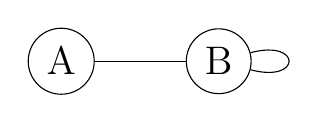
\begin{tikzpicture}[-,auto,node distance=2cm,main node/.style={circle,draw,font=\Large}]
        \tikzset{every loop/.style={}}
        \node[main node] (1) {A};
        \node[main node] (2) [right of=1] {B};
        \path
            (1) edge (2)
            (2) edge[loop right] (2);
    \end{tikzpicture} \linebreak \linebreak
    $d(B) = 3$
\end{flushleft}
\subparagraph{\large Kontextfreie Grammatik}
\normalsize
\begin{flushleft}
    \begin{itemize}
        \item \textcolor{red}{$N$} sind alle \textcolor{red}{Nichtterminalsymbole}
        \item \textcolor{red}{$T$} sind alle \textcolor{red}{Terminalsymbole}
        \item $N \cap T = \emptyset$
        \item \textcolor{red}{$S$} ist der \textcolor{red}{Start} und $S \in N$
        \item \textcolor{red}{$P$ Produktionen}, endliche Menge und $P \in N \times V^\ast$
        \begin{itemize}
            \item $V = N \cup T$ die Menge aller Symbole
            \item Für jeder $(X,w) \in P $ schreibt man $X \rightarrow w$
            \item Man "ersetz" $P$ durch $w$
        \end{itemize}
        Bei einem \textcolor{red}{Ableitungsschritt} wird ein Terminalsymbol durch abgeleitet. Dieser wird dann mit "$\Rightarrow$" dargestellt, nicht mit Implikations verwechseln!
        \linebreak \linebreak Bsp.: \linebreak
        $G = (\{X\},\{$\textcolor{blue}{a},\textcolor{blue}{b}$\},X,P)$ mit $ P = \{X \rightarrow \epsilon,X \rightarrow $\textcolor{blue}{a}$X$\textcolor{blue}{b}$\}$ \linebreak
        \linebreak
        Dann gilt zB.: \textcolor{blue}{aba}$X$\textcolor{blue}{ba}$XXXX \Rightarrow$  \textcolor{blue}{aba}$X$\textcolor{blue}{baa}$X$b$XXX$ als Ableitungsschritt.
        (Man ersetzt das $X$ nach \textcolor{blue}{ba} mit \textcolor{blue}{a}$X$\textcolor{blue}{b}) \linebreak
        \linebreak
        Man kann auch einfach mit einem Index angeben, wie viele Ableitungsschritt getätigt werden. \linebreak
        $\Rightarrow^2$ aber auch $u \Rightarrow^\ast v$ wenn $v$ aus $u$ ableitbar ist. $\Rightarrow^0$ ist einfach wieder das selbe.
        \begin{itemize}
            \item Eine \textcolor{red}{Grammatik} erzeugt eine \textcolor{red}{formale Sprache}, also einfach alle Wörter die man aus einer Grammtik ableiten kann.
            \item $G = (N,T,S,P)$ erzeugt die formale Sprache $L(G) = \{w \in T^* | S \Rightarrow^\ast w\}$
            \item Diese formalen Sprachen heißen \textcolor{red}{kontextfrei}
        \end{itemize}
    \end{itemize}
\end{flushleft}
\subparagraph{\large Zweierkomplement und Zahlensysteme}
\normalsize
\begin{flushleft}
    Wir können jedes Zahlensystem einer Basis als Alphabet auffassen: \\
    zB.: $Z_{10} = \{0,1,2,3,4,5,6,7,8,9\}$ ist das Alphabet für Dezimalzahlen.
    Wir können diese Ziffern und eine Ziffernfolge (Wort) nun umrechnen in unserer bekanntes Dezimalsystem:
    \begin{align*}
        &Num_{10}(x_{k - 1} \cdots x_1x_0) \\
        =&10^{k-1} \cdot num_{10}(x_{k-1}) + \cdots + 10^1 \cdot num_{10}(x_1) + 10^0 \cdot num_{10}(x_0)
    \end{align*}
    Das sieht jetzt deutlich komplizierter aus als es eigentlich ist. Deswegen machen wir einfach ein kleines Beispiel: \\
    Wir nehmen das Wort (Ziffernfolge) $w = 324 \in Z_{10}^{\ast}$, nun schreiben scheiben wir dieses Wort in unsere Formel:
    \begin{align*}
        Num_{10}(324) &= 10^2 \cdot num_{10}(3) + 10^1 \cdot num_{10}(2) + 10^0 \cdot num_{10}(4) \\
        &= 10^2 \cdot 3 + 10 \cdot 2 + 1 \cdot 4 = 324
    \end{align*}
    Jetzt fragt man sich warum man das überhaupt so umständlich rechnet? Man kann das doch ablesen?
    Natürlich ist uns im bekannten Dezimalsystem die Umrechnung nur einleuchtend und ablesbar. Wir haben das Dezimalsystem über 10 Jahre in der Schule kennen gelernt.
    Da wir jetzt aber gesehen habe wie es funktioniert können wir auch andere Zahlensysteme ausprobieren: \\
    zB.: Wir nehmen die Ziffernfolge $w = 1010 \in Z_2^{\ast}$. Die Umrechnung sieht wie folgt aus:
    \begin{align*}
        Num_2(1010) &= 2^3 \cdot num_2(1) + 2^2 \cdot num_2(0) + 2^1 \cdot num_2(1) + 2^0 \cdot num_2(0) \\
        &= 16 \cdot 1 + 8 \cdot 0 + 4 \cdot 1 + 1 \cdot 0 = 20
    \end{align*}
    Das kann man jetzt immer weiter führen mit allen möglichen Basen:
    \begin{itemize}
        \item $Z_{8} = \{0,1,2,3,4,5,6,7,8\}$
        \item $Z_{16} = \{0,1,2,3,4,5,6,7,8,9,A,B,C,D,E,F\}$
        Wobei dann hier $num_{16}(A) = 10$, $num_{16}(B) = 11$, \dots und so weiter sind.
        \item Kurzgesagt ist $Num_{base}(w)$ einfach die Übersetzung der Ziffernfolge $w$ eines Zahlensystems der Basis $base$ in das uns bekannte Dezimalsystem.
        \item $num(\epsilon)$ ist immer $0$
    \end{itemize}
    Nun haben wir auch noch die Umkehrfunktion zu $num_k$, nämlich $repr_k$. Dem zu Folge ist für $i\in \mathbb{Z}_k$ $repr_k(i)$ das entsprechende Zeichen.
    Die Definition für $Repr_k: \mathbb{N}_0 \rightarrow \mathbb{Z}_k$ ist nun folgende:
    \begin{align*}
        n \mapsto \begin{cases}
            repr_k(n) & \text{falls } n < k \\
            Repr_k(n \textbf{ div } k) \cdot repr_k(n \textbf{ mod } k) & \text{falls } n \geq k
        \end{cases}
    \end{align*}
    Lemma: $Num_k$ ist linksinverse zu $Repr_k$, also
    \begin{align*}
        Num_k(Repr_k(n)) = n
    \end{align*}

    \vspace{1cm}
    \textbf{Zweierkomplement:} \\
    Das Zweierkomplement hat die Besonderheit eines Vorzeichen-Bits (Sign-Bit) was einfach das Vorzeichen der Dezimalzahl ist und ist immer das höchstwertige Bit (Das erste :D).
    Dabei markiert 1 eine negative Dezimalzahl und 0 eine positive Dezimalzahl. \\
    zB. 00011010 ist positiv und 11100110 ist negativ \\
    \vspace{0.5cm}
    Zur Umrechnung können wir uns einen einfachen Trick merken:
    \begin{itemize}
        \item Wenn das Sign-Bit 0 ist rechnen wir einfach nur die Binärzahl aus:
        \begin{align*}
            00011010 &= 2^6 \cdot 0 + 2^5 \cdot 0 + 2^4 \cdot 1 + 2^3 \cdot 1 + 2^2 \cdot 0 + 2^1 \cdot 1 + 2^0 \cdot 0 \\
            &= 16 + 8 + 2 = 26
        \end{align*}
        \item Wenn das Sign-Bit 1 ist rechnen wir zunächst die maximal darstellbare Dezimalzahl für diese Binärzahl aus (Alles auf 1 setzen)
        und rechnen da nochmal 1 drauf, das ergibt unsere Wertigkeit.
        Das kann man sich auch einfach merken (In unserem 8-bit Fall ist die Wertigkeit immer 128).
        Dann rechnen wir noch den Dezimalwert unserer Binärzahl aus und ziehst dann die Wertigkeit ab (Da wir ja eine 1 als Sign-Bit haben): \linebreak
        \linebreak Zunächst berechnen wir die Wertigkeit von 11100110:
        \begin{align*}
            1111111 + 1 = 2^7 + 2^6 + 2^5 + 2^4 + 2^3 + 2^2 + 2 + 1 + 1 = 128
        \end{align*}
        Dann rechnen wir einfach die Dezimalwert unserer Binärzahl aus:
        \begin{align*}
            11100110 &= 64 + 32 + 4 + 2 = 102
        \end{align*}
        Und nun ziehen wir einfach die Wertigkeit ab:
        \begin{align*}
            102 - 128 = -26
        \end{align*}
        Wenn man die Wertigkeiten nicht jedes mal ausrechnen will,
        hier eine Tabelle: \linebreak \linebreak
        \begin{tabular}{|c|c|c|c|c|c|c|c|}
            \hline
            Wertigkeit & 256 & 128 & 64 & 32 & 16 & 8 & 4 \\
            \hline
            Bitfolge & 9 Bit & 8 Bit & 7 Bit & 6 Bit & 5 Bit  & 4 Bit & 3 Bit \\
            \hline
        \end{tabular}
    \end{itemize}
\end{flushleft}
\subparagraph{\large Turing-Maschinen}
\normalsize
\begin{flushleft}
    Eine Turingmaschine ist im Grunde einfach nur ein spezieller Automat. Die Besonderheit der Turingmaschinen ist das "Speicherband", der
    "Schreib-Lese-Kopf" und die Anweisungen für den Schreib-Lese-Kopf in der Ausgabe.
    \begin{itemize}
        \item Das Speicherband ist in einzelne Zellen eingeteilt (Wie ein Array) das nach links und rechts "unendlich" ist.
        \item Eine leere Zelle wird mit dem Symbol $\square$ markiert.
        \item Der Schreib-Lese-Kopf zeigt immer auf eine Zelle im Speicherband und auf einen Zustand in der Turingmaschine.
        \item Wie auch bei Automaten gibt es akzeptierende und nicht akzeptierende Zustände.
        \item Die Eingabe ist der Inhalt der Zelle, auf welche der Schreib-Lese-Kopf zeigt, und die Ausgabe wird eben in diese nun geschrieben. Dabei gibt es in der Ausgabe zwei Anweisungen:
        \begin{itemize}
            \item $L$ Der Schreib-Lese-Kopf wird um eins nach links verschoben.
            \item $R$ Der Schreib-Lese-Kopf wird um eins nach rechts verschoben.
            \item $0$ Der Schreib-Lese-Kopf bleibt einfach in der Zelle.
        \end{itemize}
        \item Eine Turingmaschine muss nicht jedes Szenario abhandeln können. Im Falle eines unbehandelten Falles bleibt die Turingmaschine einfach stehen.
        \item Wenn man zB. nun ein Wort in die Turingmaschine geben möchte, muss man dieses Wort einfach auf das Speicherband schreiben.
    \end{itemize}
    \includegraphics[width=0.8\textwidth]{simple_turing.png} \\
    Hier sieht man eine simple Turingmaschine mit einem einzigen Zustand $Z$. Die Zellen unter dem Zustand sind das Speicherband mit der Eingabe. Der Pfeil symbolisiert den Schreib-Lese-Kopf.
    Aktuell befindet sich die Turingmaschine im Zustand $Z$ und liest/schreibt in die erste Zelle des Speicherbandes.
    \linebreak \linebreak
    Jede Turingmaschine kann zu einer Tabelle umgeschrieben, das Beispiel sollte fürs Verständnis ausreichen:
    \includegraphics[width=0.8\textwidth]{turing_table.png} \\
    Die rechte Spalte repräsentiert die mögliche Eingabe ($1$ oder $\square$). Die obere Zeile sind die verschiedenen Zustände ($A,B,C,H$).
    In die Tabelle wird dann Eingetragen was welcher Zustand für welche Eingabe macht. \\
    zB. für die Eingabe $\square$ in Zustand $A$, schreibt der Schreib-Lese-Kopf eine $1$ in die Zelle des Speicherbandes, das $R$ bewegt den Schreib-Lese-Kopf eins nach rechts und der Zustand wechselt zu Zustand $B$.
\end{flushleft}
\subparagraph{\large Relationen}
\normalsize
\begin{flushleft}
    Eine Relation $\mathbf{R}$ kann folgende Eigenschaften haben:
\begin{itemize}
    \item \textbf{Transitivität}, wenn aus $x\mathbf{R}y$ und $y\mathbf{R}z$ auch $x\mathbf{R}z$ folgt.
    \item \textbf{Reflexivität}, wenn $x\mathbf{R}x$ gilt.
    \item \textbf{Symmetrie}, wenn $x\mathbf{R}y \Rightarrow y\mathbf{R}x$.
\end{itemize}
Hat eine Relation alle der drei oben genannten Eigenschaften, wird diese Relation auch als Äuqivalenzrelation bezeichnet.
Die bekannteste Äuqivalenzrelation ist wohl "$=$".
\end{flushleft}
\end{document}
